\documentclass[11pt]{article}
\usepackage[textwidth=18.0cm, textheight=23.0cm, top=2.0cm]{geometry}
\usepackage{pst-all}
\usepackage{amssymb}
\usepackage{tikz}
\usepackage{underscore}\begin{document}
\pagestyle{empty}


ClassName: \underline{\textbf{Class_05.2bp-14}}
\par
BinSize: \underline{\textbf{100 × 100}}
\par
ReduceSize: \underline{\textbf{100 × 100}}
\par
TypeNum: \underline{\textbf{40}}
\par
Num: \underline{\textbf{40}}
\par
OutS: \underline{\textbf{140000}}
\par
InS: \underline{\textbf{119011}}
\par
Rate: \underline{\textbf{0.850}}
\par
UB: \underline{\textbf{14}}
\par
LB0: \underline{\textbf{13}}
\par
LB: \underline{\textbf{14}}
\par
LBWithCut: \underline{\textbf{14}}
\par
NodeCut: \underline{\textbf{0}}
\par
ExtendedNodeCnt: \underline{\textbf{1}}
\par
GenNodeCnt: \underline{\textbf{1}}
\par
PrimalNode: \underline{\textbf{0}}
\par
ColumnCount: \underline{\textbf{77}}
\par
TotalCutCount: \underline{\textbf{0}}
\par
RootCutCount: \underline{\textbf{0}}
\par
LPSolverCnt: \underline{\textbf{64}}
\par
PricingSolverCnt: \underline{\textbf{64}}
\par
BranchAndBoundNum: \underline{\textbf{1}}
\par
isOpt: \underline{\textbf{true}}
\par
TimeOnInitSolution: \underline{\textbf{600.000 s}}
\par
TimeOnPrimal: \underline{\textbf{0.000 s}}
\par
TimeOnPricing: \underline{\textbf{5.141 s}}
\par
TimeOnRmp: \underline{\textbf{0.109 s}}
\par
TotalTime: \underline{\textbf{605.579 s}}
\par
\newpage



\begin{tikzpicture}[shorten >=1pt,scale=1.0,every node/.style={scale=1.0},->]
\tikzstyle{vertex}=[circle,fill=black!25,minimum size=14pt,inner sep=0pt]
\filldraw[fill=gray!40!white, draw=black] (0,0) rectangle (15.0,15.0);
\foreach \name/\x/\y/\w/\h in {100x95/0.0/0.0/15.0/14.25}
\filldraw[fill=white!40!white, draw=black] (\x,\y) rectangle node[draw] (\name) {\name} ++(\w,\h);
\end{tikzpicture}


w =100 , h =95 , x =0 , y =0 , v =9500
\par
\newpage


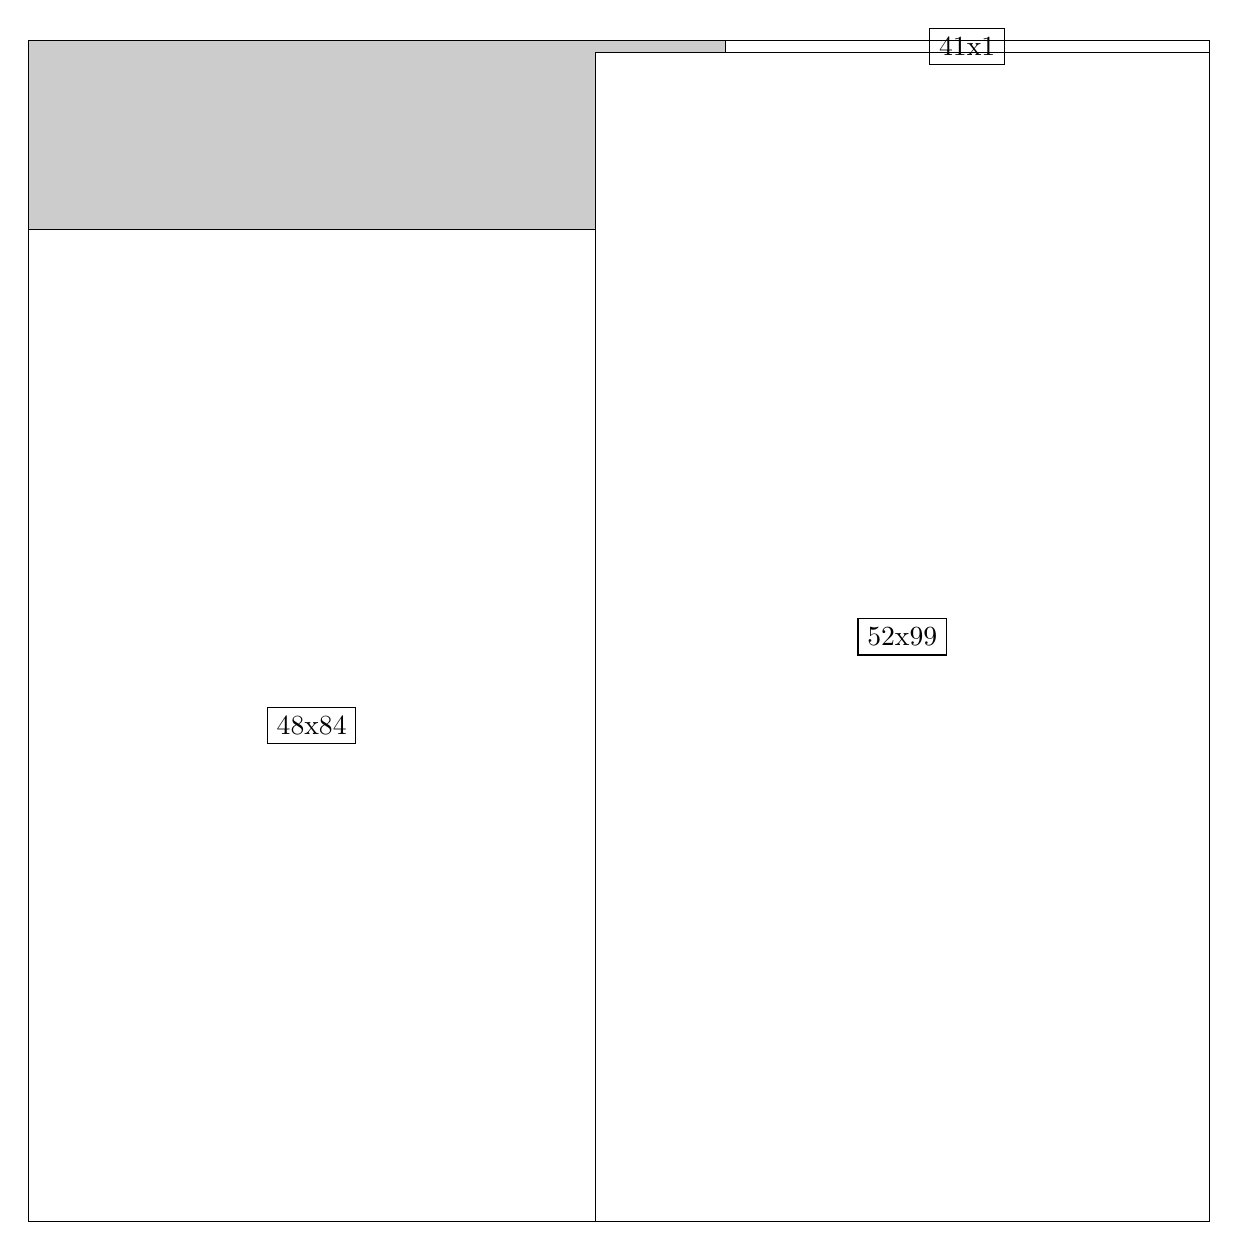
\begin{tikzpicture}[shorten >=1pt,scale=1.0,every node/.style={scale=1.0},->]
\tikzstyle{vertex}=[circle,fill=black!25,minimum size=14pt,inner sep=0pt]
\filldraw[fill=gray!40!white, draw=black] (0,0) rectangle (15.0,15.0);
\foreach \name/\x/\y/\w/\h in {52x99/7.199999999999999/0.0/7.8/14.85,41x1/8.85/14.85/6.1499999999999995/0.15,48x84/0.0/0.0/7.199999999999999/12.6}
\filldraw[fill=white!40!white, draw=black] (\x,\y) rectangle node[draw] (\name) {\name} ++(\w,\h);
\end{tikzpicture}


w =52 , h =99 , x =48 , y =0 , v =5148
\par
w =41 , h =1 , x =59 , y =99 , v =41
\par
w =48 , h =84 , x =0 , y =0 , v =4032
\par
\newpage


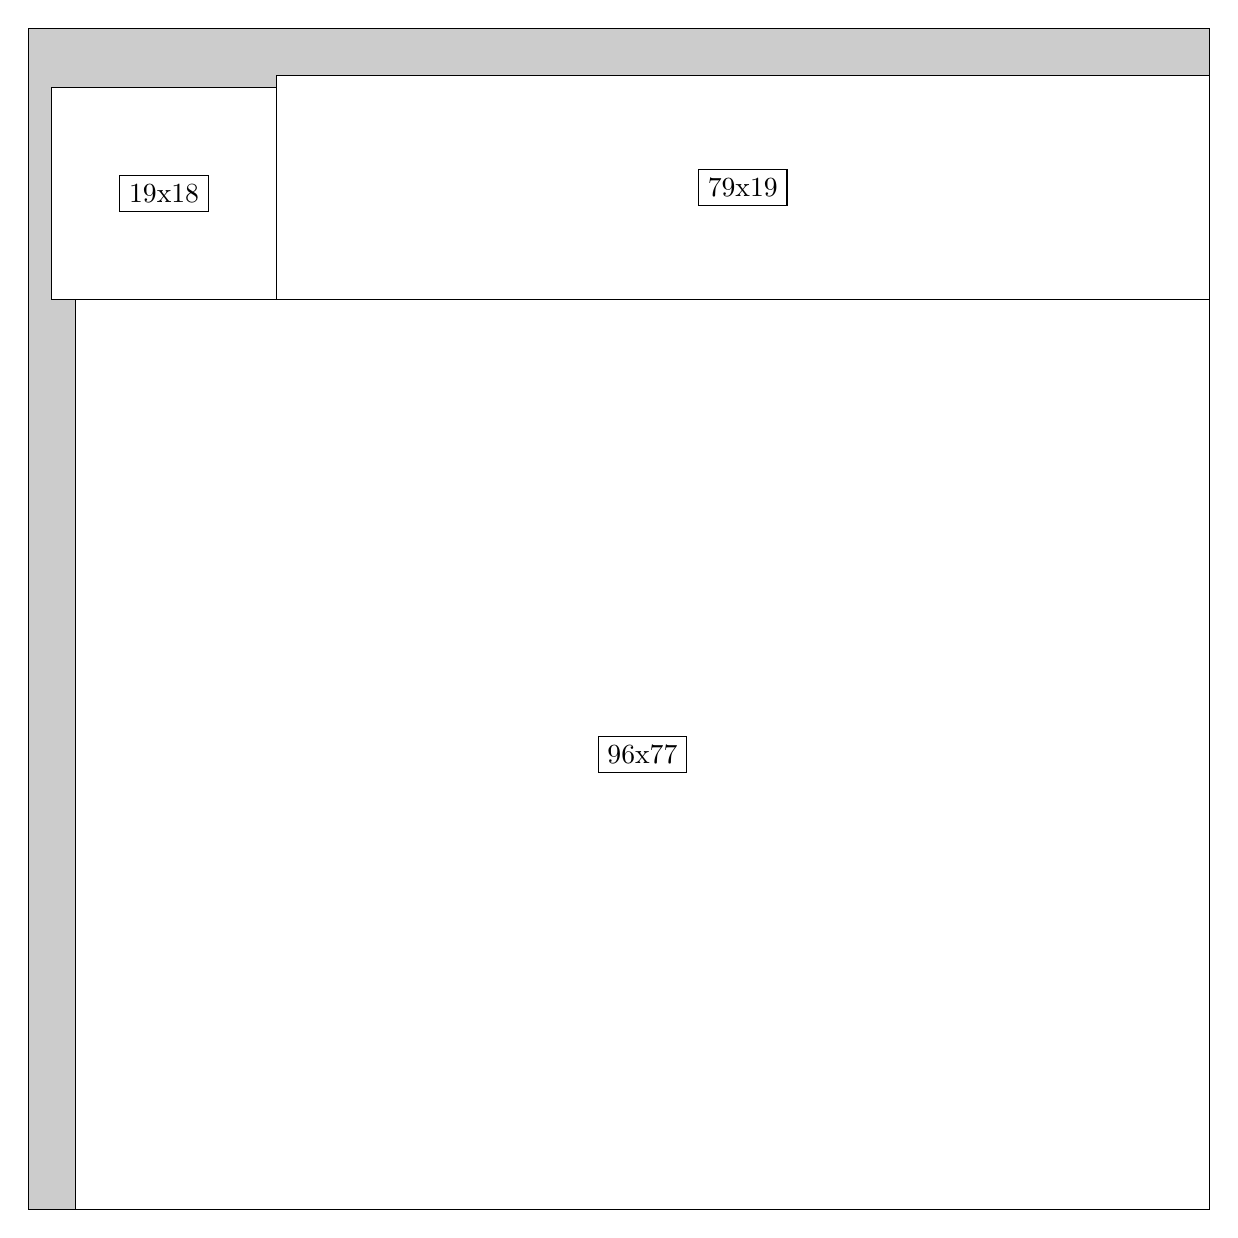
\begin{tikzpicture}[shorten >=1pt,scale=1.0,every node/.style={scale=1.0},->]
\tikzstyle{vertex}=[circle,fill=black!25,minimum size=14pt,inner sep=0pt]
\filldraw[fill=gray!40!white, draw=black] (0,0) rectangle (15.0,15.0);
\foreach \name/\x/\y/\w/\h in {96x77/0.6/0.0/14.399999999999999/11.549999999999999,79x19/3.15/11.549999999999999/11.85/2.85,19x18/0.3/11.549999999999999/2.85/2.6999999999999997}
\filldraw[fill=white!40!white, draw=black] (\x,\y) rectangle node[draw] (\name) {\name} ++(\w,\h);
\end{tikzpicture}


w =96 , h =77 , x =4 , y =0 , v =7392
\par
w =79 , h =19 , x =21 , y =77 , v =1501
\par
w =19 , h =18 , x =2 , y =77 , v =342
\par
\newpage


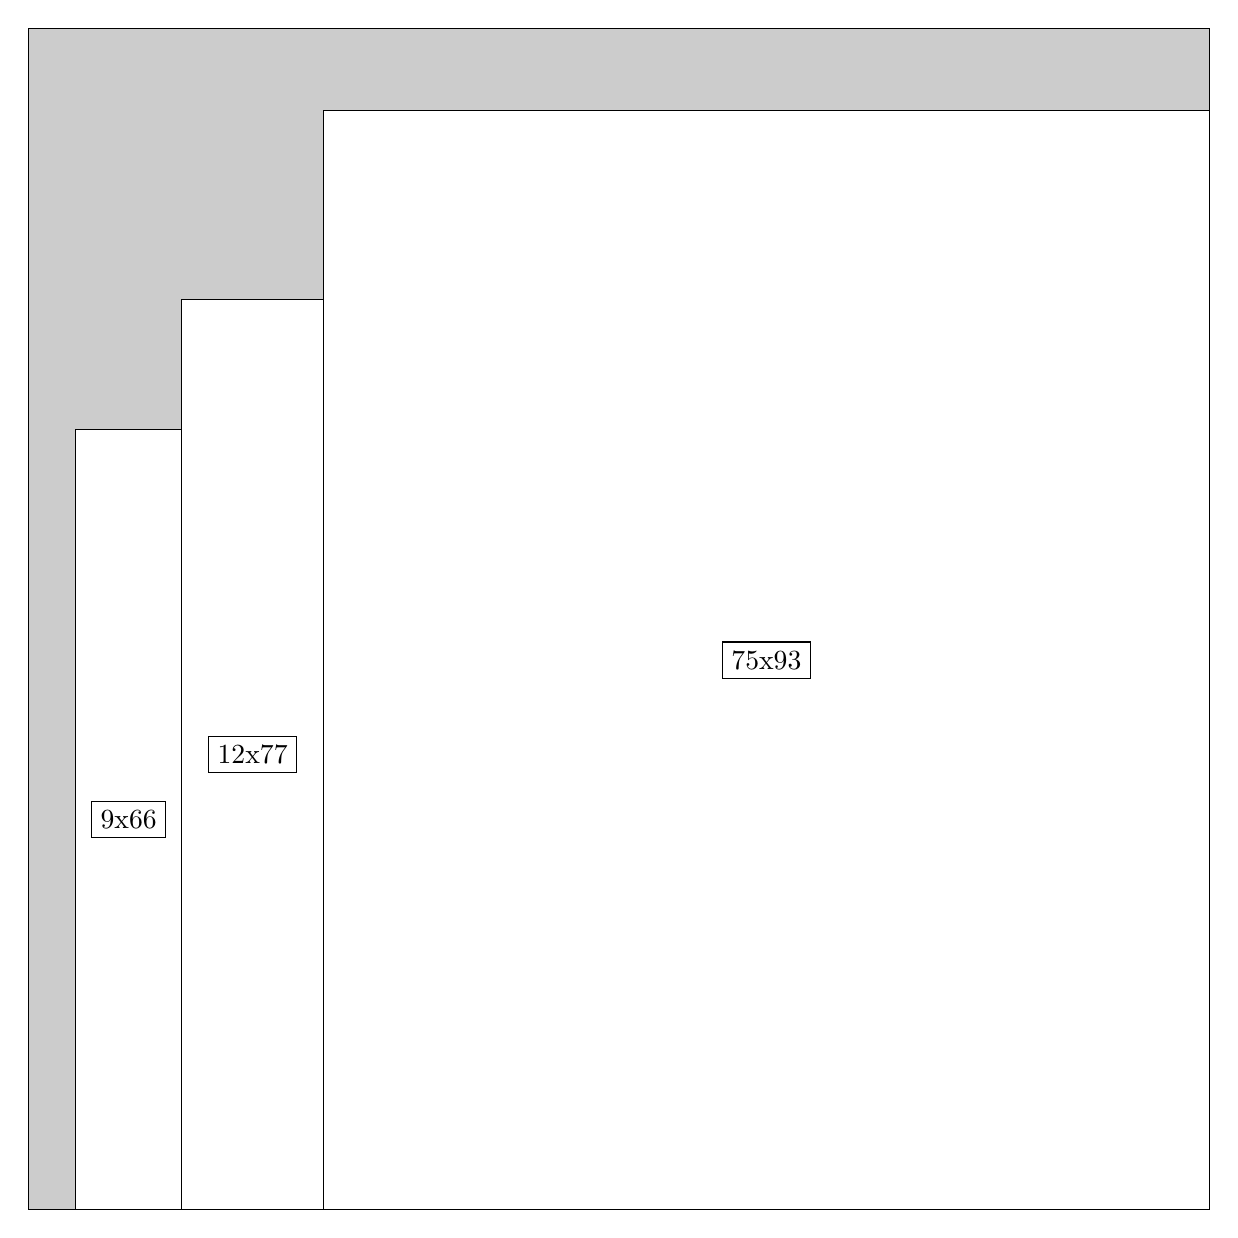
\begin{tikzpicture}[shorten >=1pt,scale=1.0,every node/.style={scale=1.0},->]
\tikzstyle{vertex}=[circle,fill=black!25,minimum size=14pt,inner sep=0pt]
\filldraw[fill=gray!40!white, draw=black] (0,0) rectangle (15.0,15.0);
\foreach \name/\x/\y/\w/\h in {75x93/3.75/0.0/11.25/13.95,12x77/1.95/0.0/1.7999999999999998/11.549999999999999,9x66/0.6/0.0/1.3499999999999999/9.9}
\filldraw[fill=white!40!white, draw=black] (\x,\y) rectangle node[draw] (\name) {\name} ++(\w,\h);
\end{tikzpicture}


w =75 , h =93 , x =25 , y =0 , v =6975
\par
w =12 , h =77 , x =13 , y =0 , v =924
\par
w =9 , h =66 , x =4 , y =0 , v =594
\par
\newpage


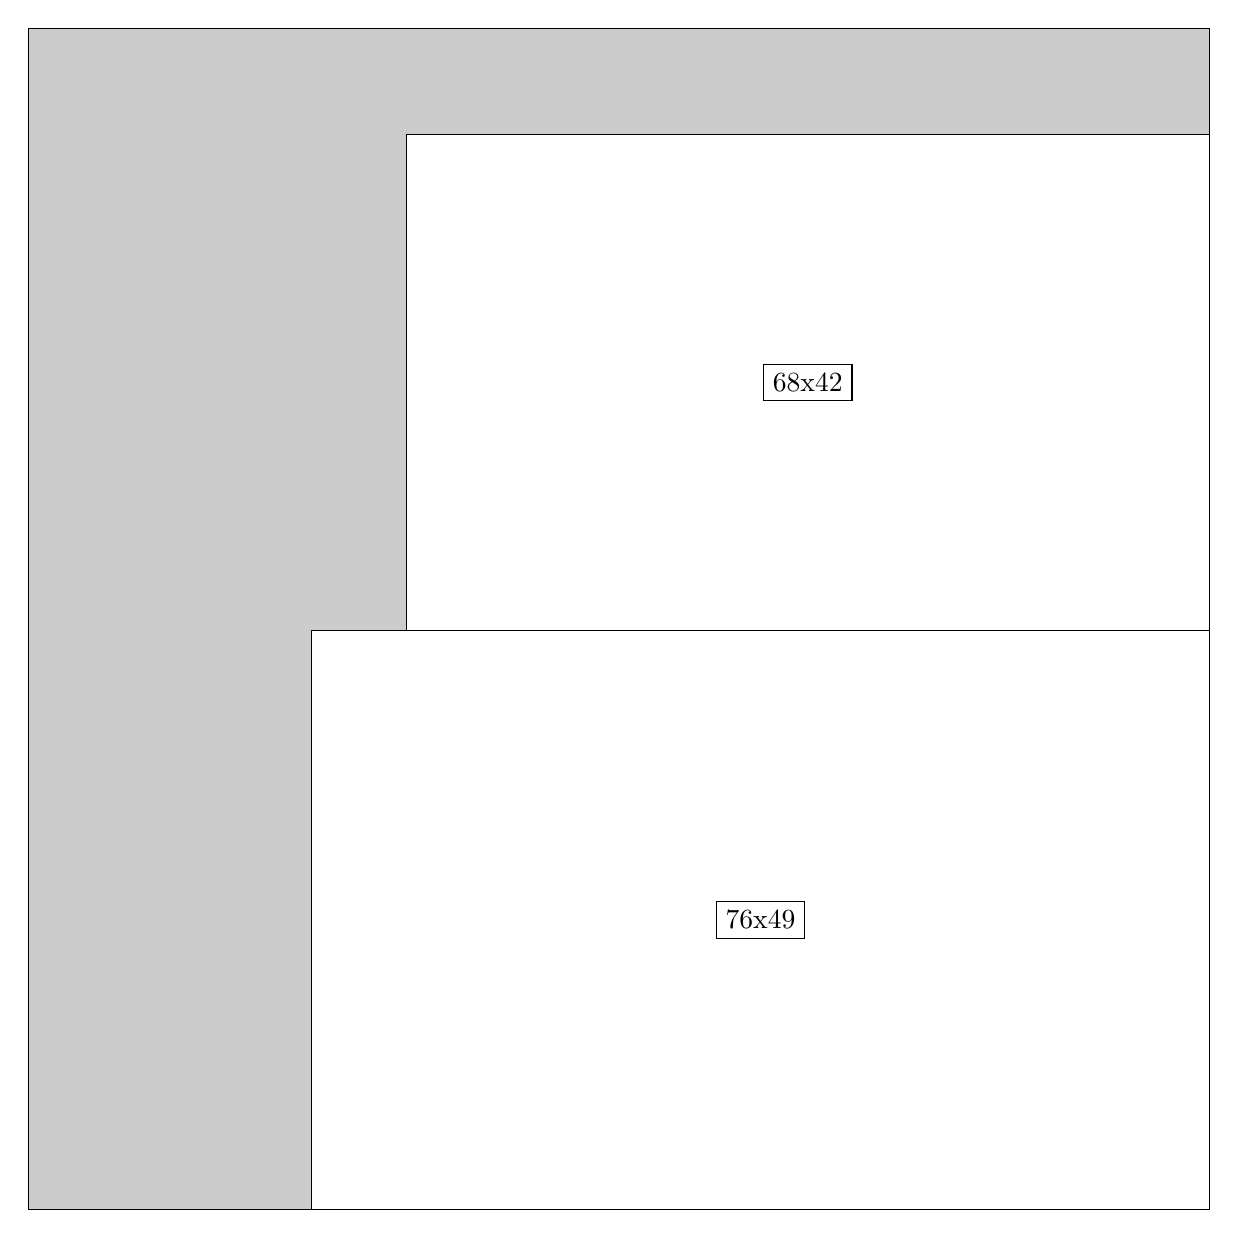
\begin{tikzpicture}[shorten >=1pt,scale=1.0,every node/.style={scale=1.0},->]
\tikzstyle{vertex}=[circle,fill=black!25,minimum size=14pt,inner sep=0pt]
\filldraw[fill=gray!40!white, draw=black] (0,0) rectangle (15.0,15.0);
\foreach \name/\x/\y/\w/\h in {76x49/3.5999999999999996/0.0/11.4/7.35,68x42/4.8/7.35/10.2/6.3}
\filldraw[fill=white!40!white, draw=black] (\x,\y) rectangle node[draw] (\name) {\name} ++(\w,\h);
\end{tikzpicture}


w =76 , h =49 , x =24 , y =0 , v =3724
\par
w =68 , h =42 , x =32 , y =49 , v =2856
\par
\newpage


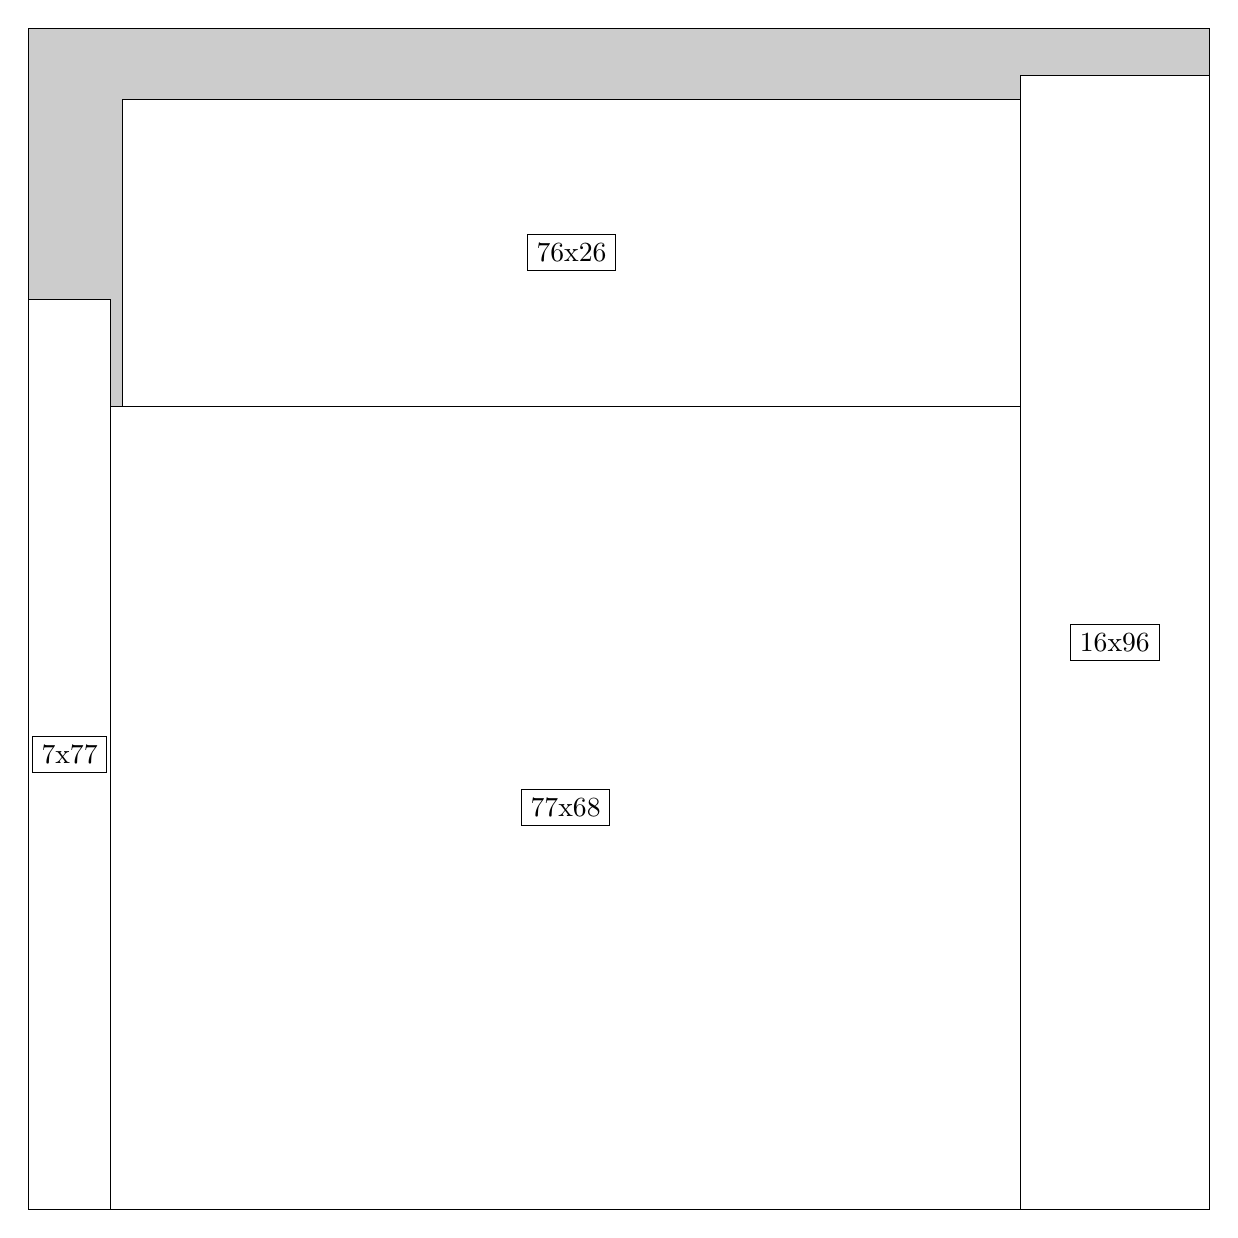
\begin{tikzpicture}[shorten >=1pt,scale=1.0,every node/.style={scale=1.0},->]
\tikzstyle{vertex}=[circle,fill=black!25,minimum size=14pt,inner sep=0pt]
\filldraw[fill=gray!40!white, draw=black] (0,0) rectangle (15.0,15.0);
\foreach \name/\x/\y/\w/\h in {16x96/12.6/0.0/2.4/14.399999999999999,77x68/1.05/0.0/11.549999999999999/10.2,76x26/1.2/10.2/11.4/3.9,7x77/0.0/0.0/1.05/11.549999999999999}
\filldraw[fill=white!40!white, draw=black] (\x,\y) rectangle node[draw] (\name) {\name} ++(\w,\h);
\end{tikzpicture}


w =16 , h =96 , x =84 , y =0 , v =1536
\par
w =77 , h =68 , x =7 , y =0 , v =5236
\par
w =76 , h =26 , x =8 , y =68 , v =1976
\par
w =7 , h =77 , x =0 , y =0 , v =539
\par
\newpage


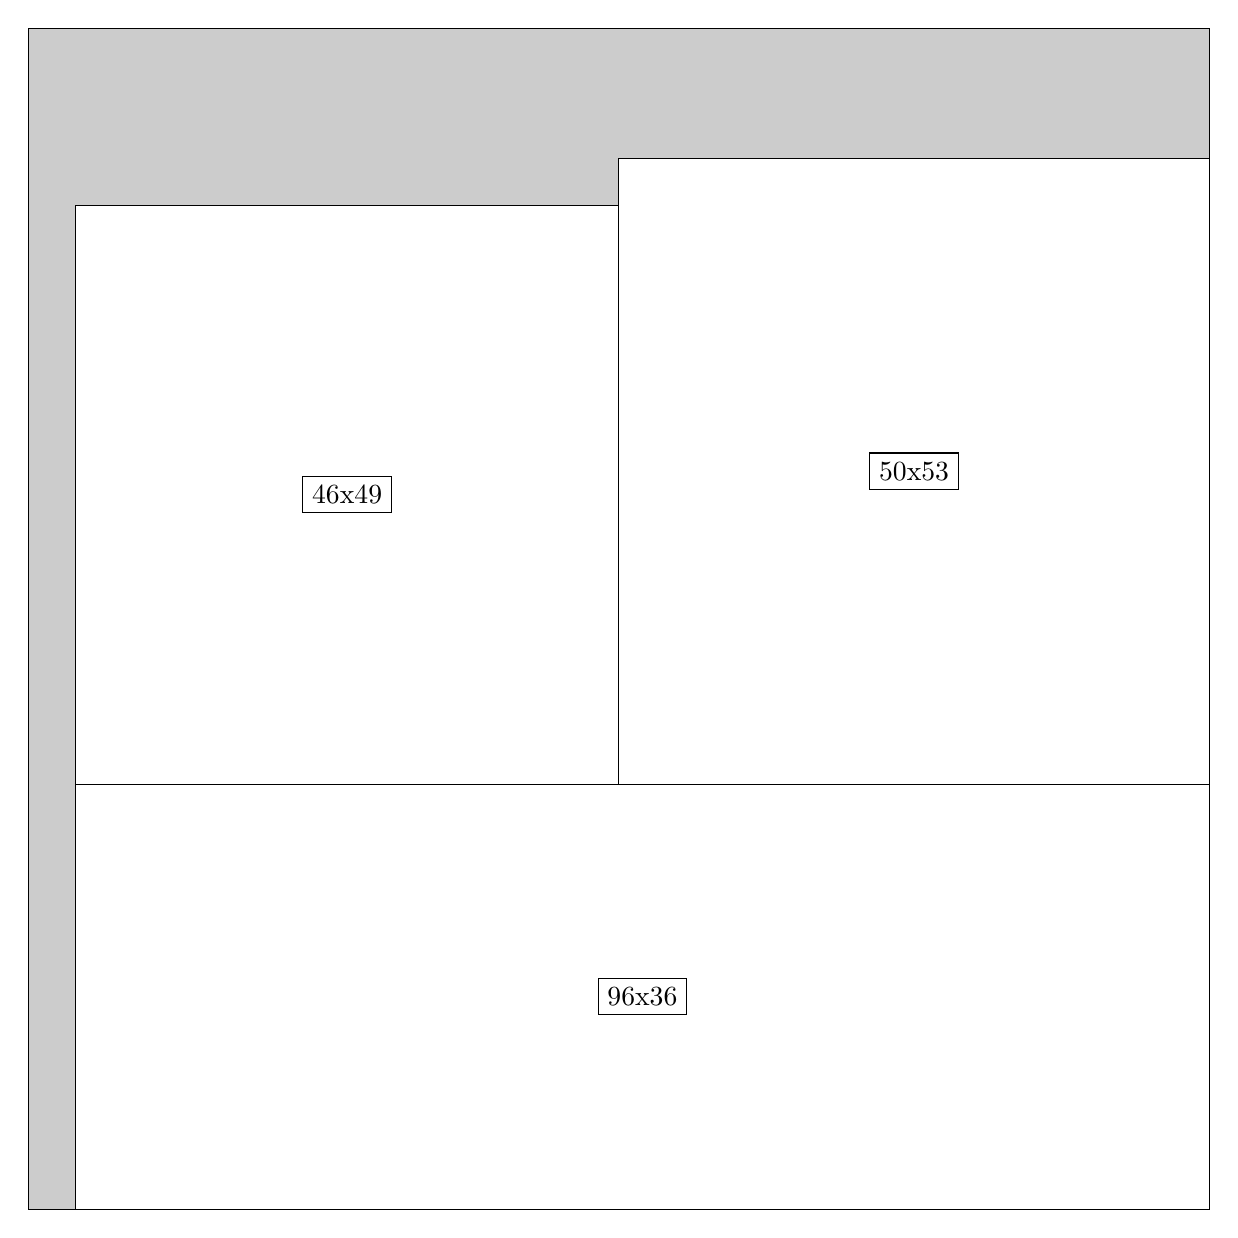
\begin{tikzpicture}[shorten >=1pt,scale=1.0,every node/.style={scale=1.0},->]
\tikzstyle{vertex}=[circle,fill=black!25,minimum size=14pt,inner sep=0pt]
\filldraw[fill=gray!40!white, draw=black] (0,0) rectangle (15.0,15.0);
\foreach \name/\x/\y/\w/\h in {96x36/0.6/0.0/14.399999999999999/5.3999999999999995,50x53/7.5/5.3999999999999995/7.5/7.949999999999999,46x49/0.6/5.3999999999999995/6.8999999999999995/7.35}
\filldraw[fill=white!40!white, draw=black] (\x,\y) rectangle node[draw] (\name) {\name} ++(\w,\h);
\end{tikzpicture}


w =96 , h =36 , x =4 , y =0 , v =3456
\par
w =50 , h =53 , x =50 , y =36 , v =2650
\par
w =46 , h =49 , x =4 , y =36 , v =2254
\par
\newpage


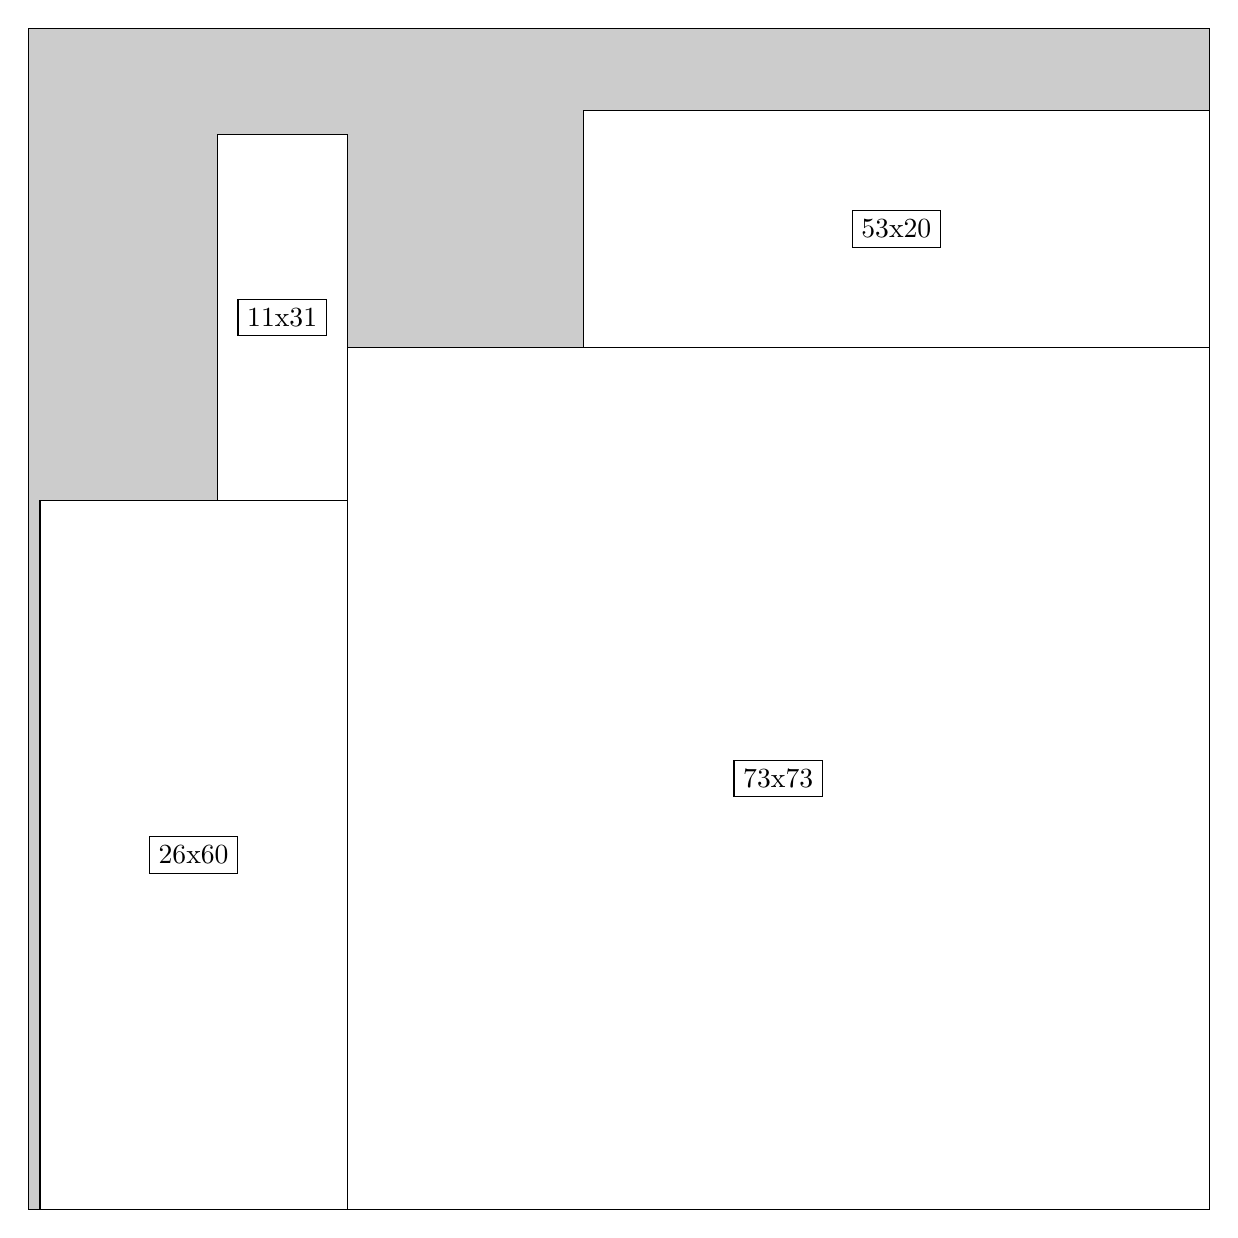
\begin{tikzpicture}[shorten >=1pt,scale=1.0,every node/.style={scale=1.0},->]
\tikzstyle{vertex}=[circle,fill=black!25,minimum size=14pt,inner sep=0pt]
\filldraw[fill=gray!40!white, draw=black] (0,0) rectangle (15.0,15.0);
\foreach \name/\x/\y/\w/\h in {73x73/4.05/0.0/10.95/10.95,53x20/7.05/10.95/7.949999999999999/3.0,26x60/0.15/0.0/3.9/9.0,11x31/2.4/9.0/1.65/4.6499999999999995}
\filldraw[fill=white!40!white, draw=black] (\x,\y) rectangle node[draw] (\name) {\name} ++(\w,\h);
\end{tikzpicture}


w =73 , h =73 , x =27 , y =0 , v =5329
\par
w =53 , h =20 , x =47 , y =73 , v =1060
\par
w =26 , h =60 , x =1 , y =0 , v =1560
\par
w =11 , h =31 , x =16 , y =60 , v =341
\par
\newpage


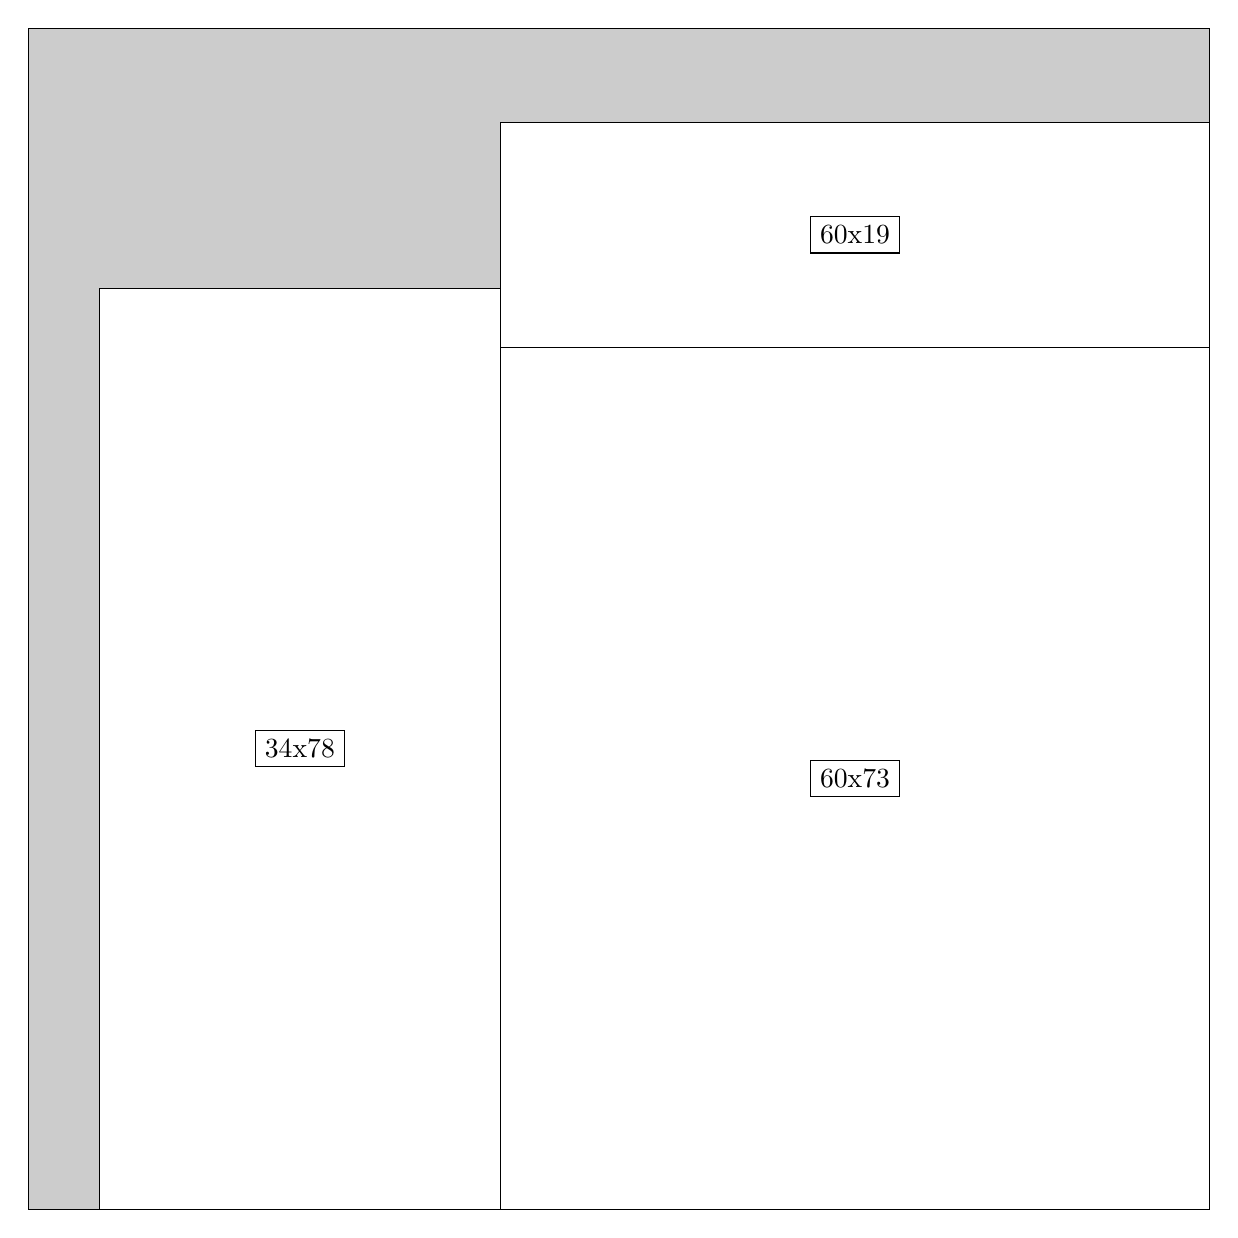
\begin{tikzpicture}[shorten >=1pt,scale=1.0,every node/.style={scale=1.0},->]
\tikzstyle{vertex}=[circle,fill=black!25,minimum size=14pt,inner sep=0pt]
\filldraw[fill=gray!40!white, draw=black] (0,0) rectangle (15.0,15.0);
\foreach \name/\x/\y/\w/\h in {60x73/6.0/0.0/9.0/10.95,60x19/6.0/10.95/9.0/2.85,34x78/0.8999999999999999/0.0/5.1/11.7}
\filldraw[fill=white!40!white, draw=black] (\x,\y) rectangle node[draw] (\name) {\name} ++(\w,\h);
\end{tikzpicture}


w =60 , h =73 , x =40 , y =0 , v =4380
\par
w =60 , h =19 , x =40 , y =73 , v =1140
\par
w =34 , h =78 , x =6 , y =0 , v =2652
\par
\newpage


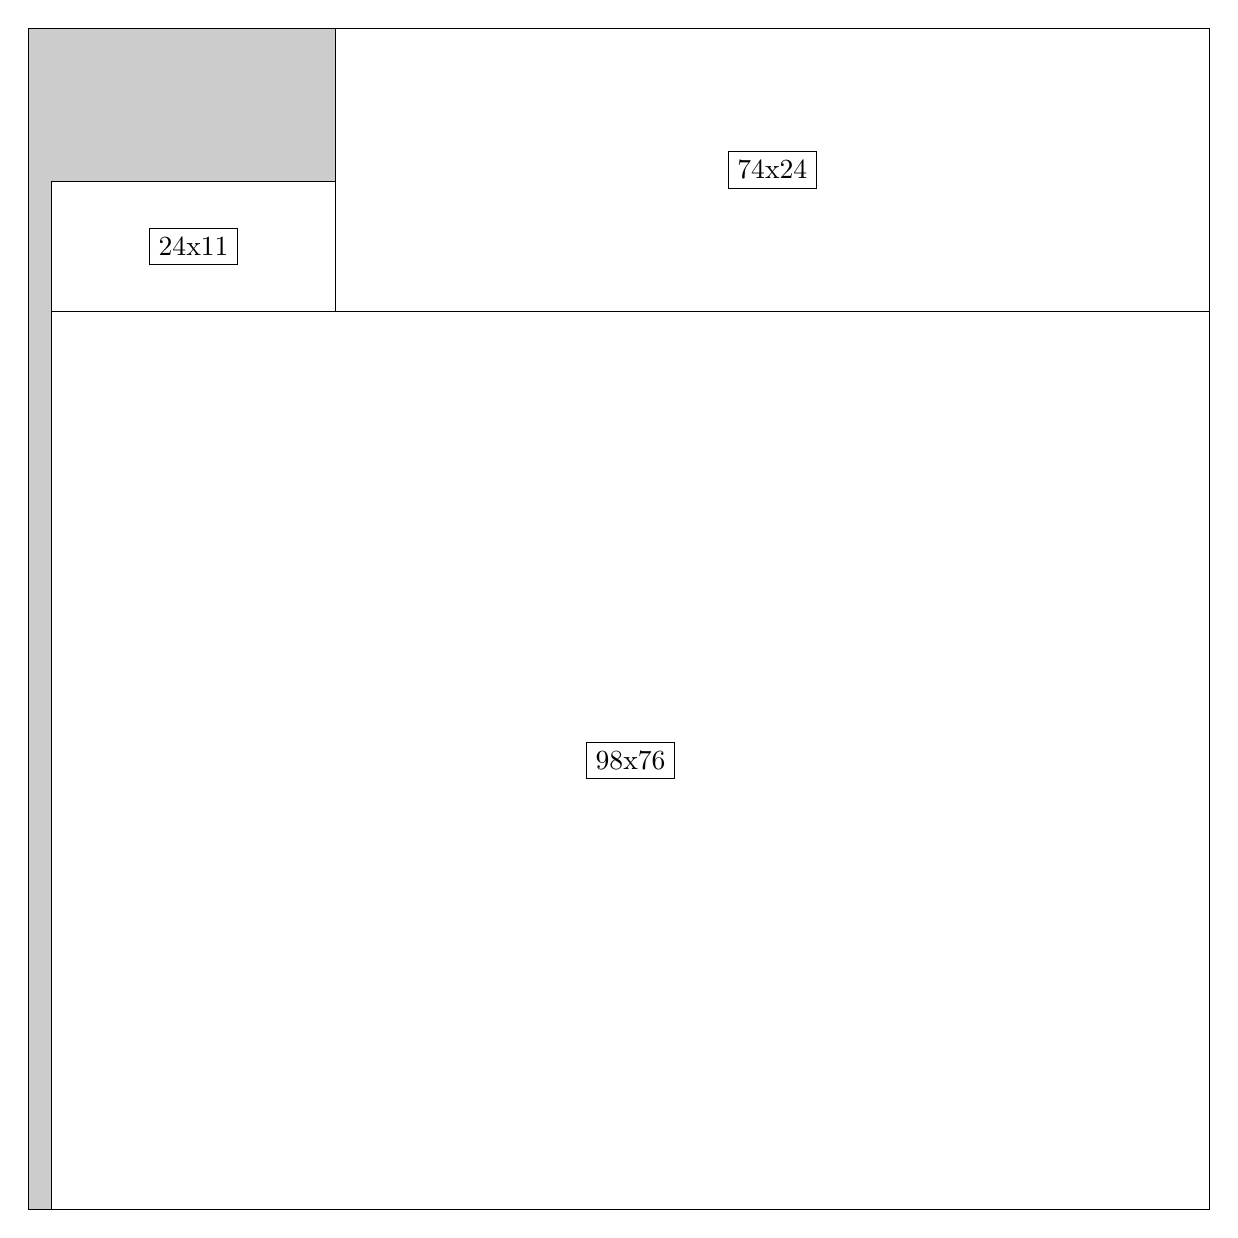
\begin{tikzpicture}[shorten >=1pt,scale=1.0,every node/.style={scale=1.0},->]
\tikzstyle{vertex}=[circle,fill=black!25,minimum size=14pt,inner sep=0pt]
\filldraw[fill=gray!40!white, draw=black] (0,0) rectangle (15.0,15.0);
\foreach \name/\x/\y/\w/\h in {98x76/0.3/0.0/14.7/11.4,74x24/3.9/11.4/11.1/3.5999999999999996,24x11/0.3/11.4/3.5999999999999996/1.65}
\filldraw[fill=white!40!white, draw=black] (\x,\y) rectangle node[draw] (\name) {\name} ++(\w,\h);
\end{tikzpicture}


w =98 , h =76 , x =2 , y =0 , v =7448
\par
w =74 , h =24 , x =26 , y =76 , v =1776
\par
w =24 , h =11 , x =2 , y =76 , v =264
\par
\newpage


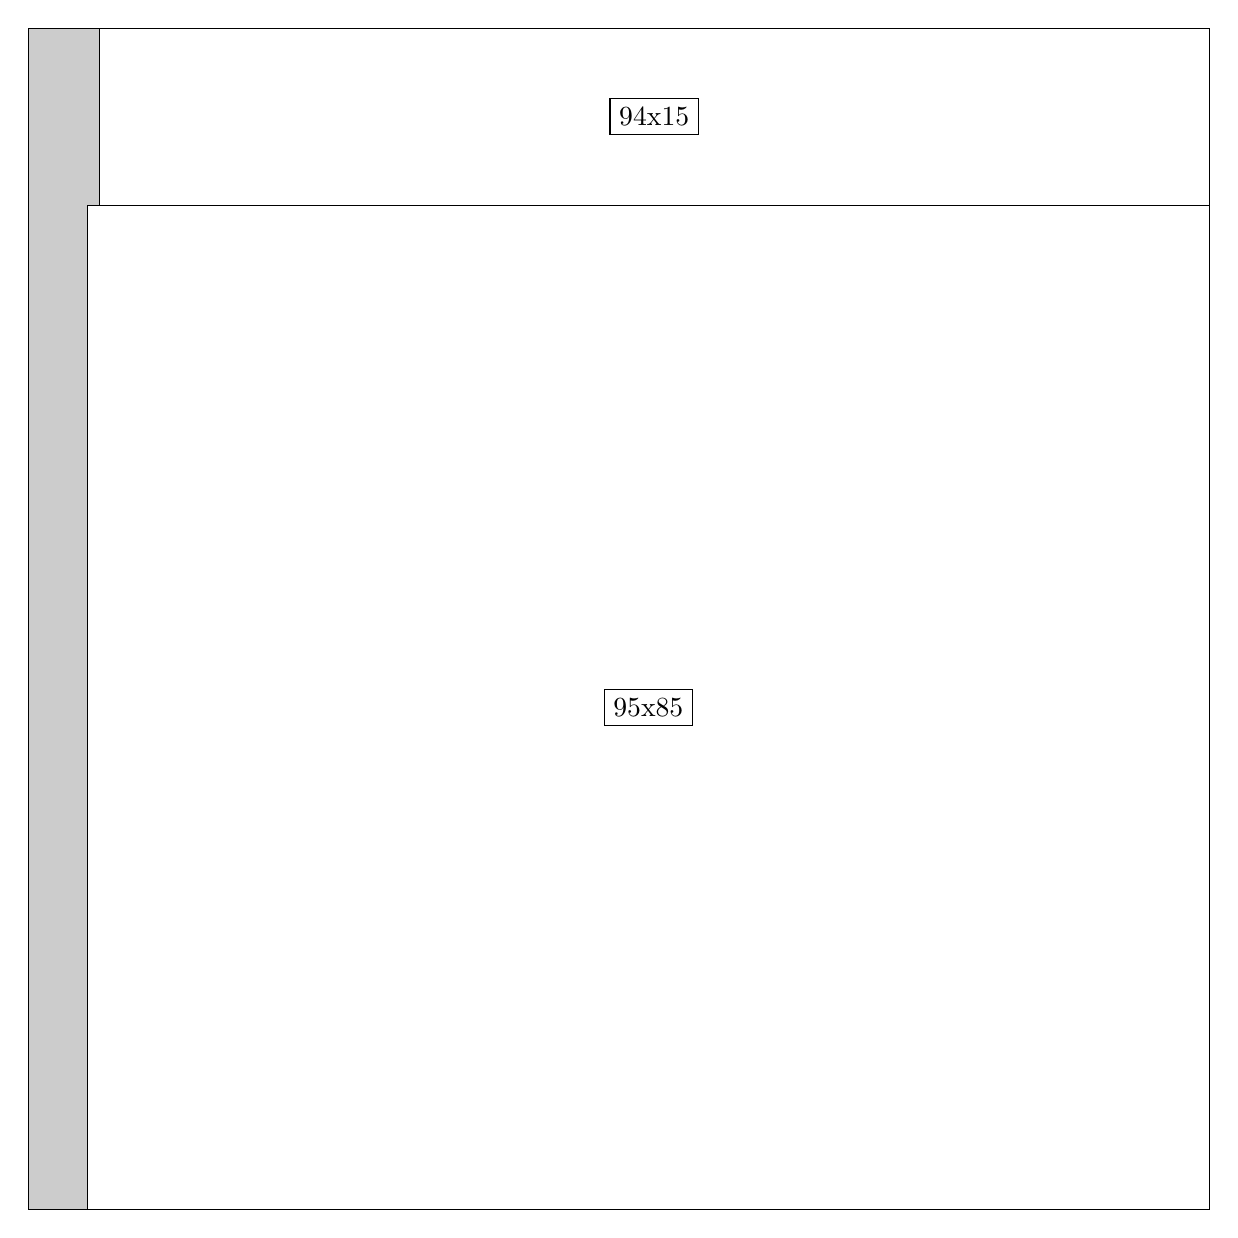
\begin{tikzpicture}[shorten >=1pt,scale=1.0,every node/.style={scale=1.0},->]
\tikzstyle{vertex}=[circle,fill=black!25,minimum size=14pt,inner sep=0pt]
\filldraw[fill=gray!40!white, draw=black] (0,0) rectangle (15.0,15.0);
\foreach \name/\x/\y/\w/\h in {95x85/0.75/0.0/14.25/12.75,94x15/0.8999999999999999/12.75/14.1/2.25}
\filldraw[fill=white!40!white, draw=black] (\x,\y) rectangle node[draw] (\name) {\name} ++(\w,\h);
\end{tikzpicture}


w =95 , h =85 , x =5 , y =0 , v =8075
\par
w =94 , h =15 , x =6 , y =85 , v =1410
\par
\newpage


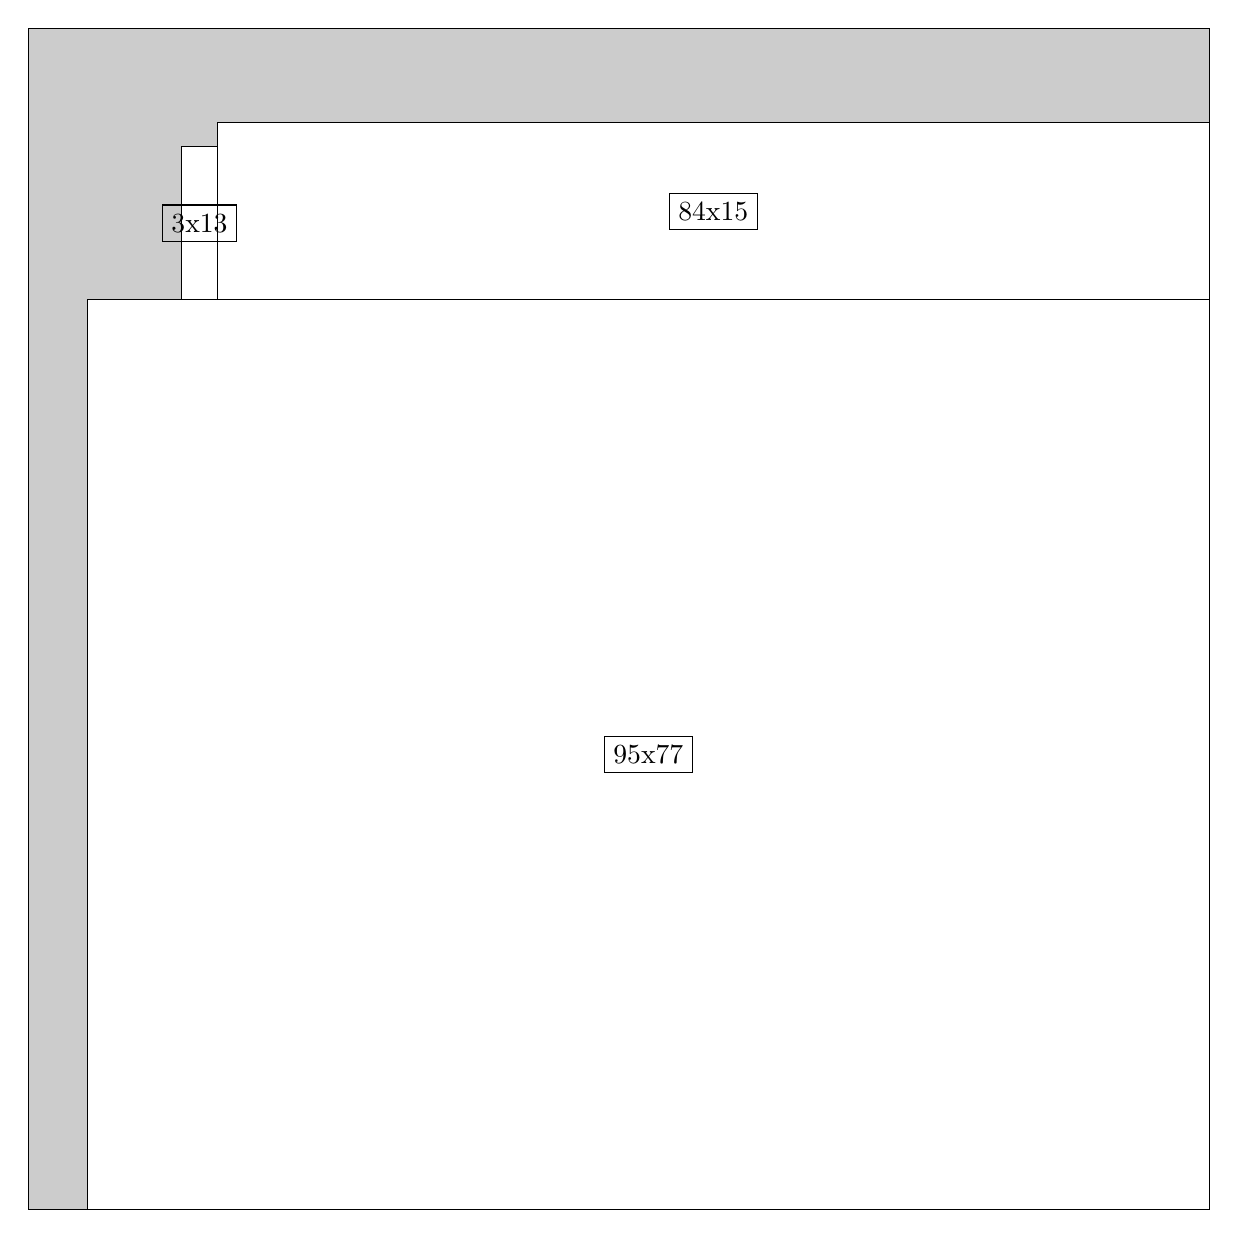
\begin{tikzpicture}[shorten >=1pt,scale=1.0,every node/.style={scale=1.0},->]
\tikzstyle{vertex}=[circle,fill=black!25,minimum size=14pt,inner sep=0pt]
\filldraw[fill=gray!40!white, draw=black] (0,0) rectangle (15.0,15.0);
\foreach \name/\x/\y/\w/\h in {95x77/0.75/0.0/14.25/11.549999999999999,84x15/2.4/11.549999999999999/12.6/2.25,3x13/1.95/11.549999999999999/0.44999999999999996/1.95}
\filldraw[fill=white!40!white, draw=black] (\x,\y) rectangle node[draw] (\name) {\name} ++(\w,\h);
\end{tikzpicture}


w =95 , h =77 , x =5 , y =0 , v =7315
\par
w =84 , h =15 , x =16 , y =77 , v =1260
\par
w =3 , h =13 , x =13 , y =77 , v =39
\par
\newpage


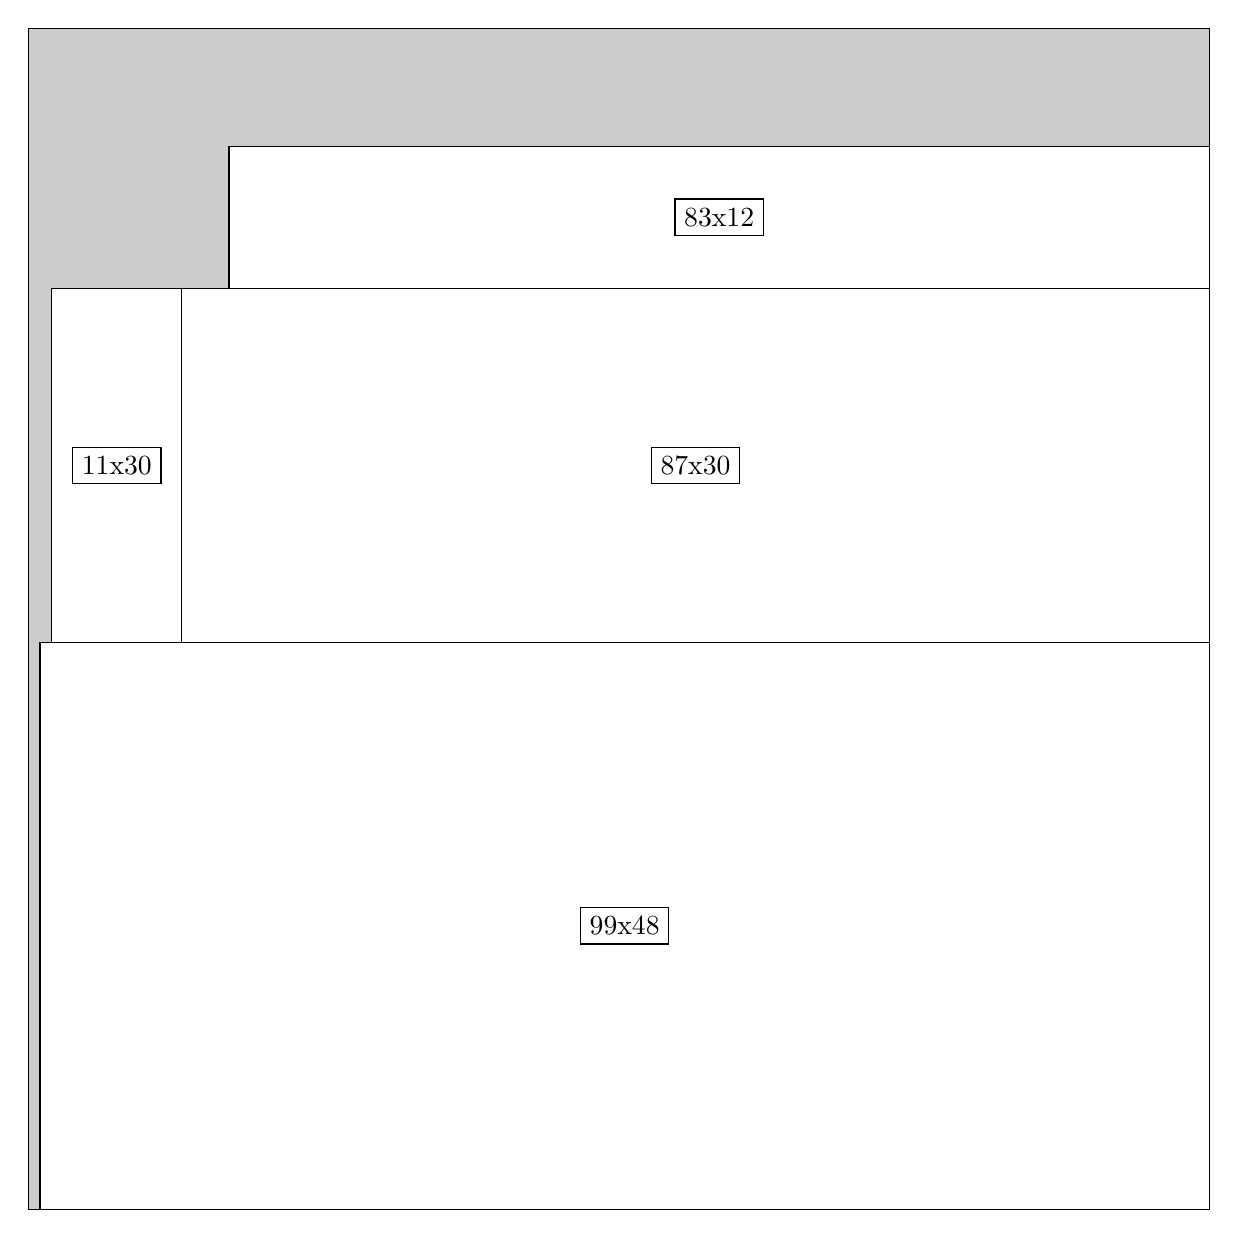
\begin{tikzpicture}[shorten >=1pt,scale=1.0,every node/.style={scale=1.0},->]
\tikzstyle{vertex}=[circle,fill=black!25,minimum size=14pt,inner sep=0pt]
\filldraw[fill=gray!40!white, draw=black] (0,0) rectangle (15.0,15.0);
\foreach \name/\x/\y/\w/\h in {99x48/0.15/0.0/14.85/7.199999999999999,87x30/1.95/7.199999999999999/13.049999999999999/4.5,83x12/2.55/11.7/12.45/1.7999999999999998,11x30/0.3/7.199999999999999/1.65/4.5}
\filldraw[fill=white!40!white, draw=black] (\x,\y) rectangle node[draw] (\name) {\name} ++(\w,\h);
\end{tikzpicture}


w =99 , h =48 , x =1 , y =0 , v =4752
\par
w =87 , h =30 , x =13 , y =48 , v =2610
\par
w =83 , h =12 , x =17 , y =78 , v =996
\par
w =11 , h =30 , x =2 , y =48 , v =330
\par
\newpage


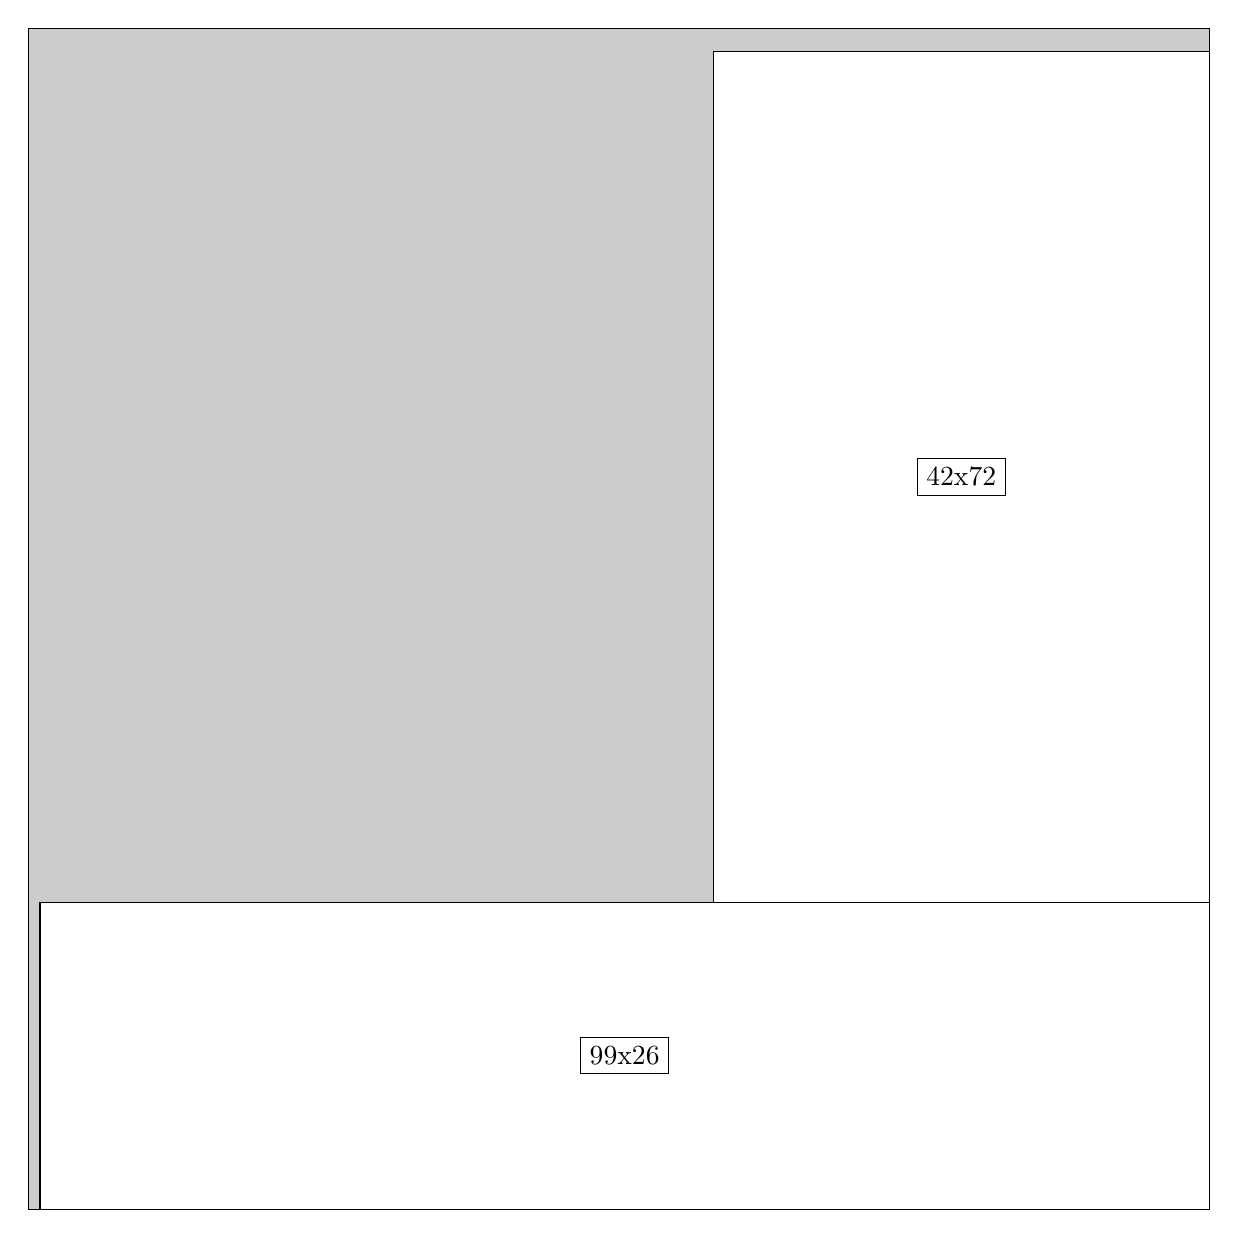
\begin{tikzpicture}[shorten >=1pt,scale=1.0,every node/.style={scale=1.0},->]
\tikzstyle{vertex}=[circle,fill=black!25,minimum size=14pt,inner sep=0pt]
\filldraw[fill=gray!40!white, draw=black] (0,0) rectangle (15.0,15.0);
\foreach \name/\x/\y/\w/\h in {99x26/0.15/0.0/14.85/3.9,42x72/8.7/3.9/6.3/10.799999999999999}
\filldraw[fill=white!40!white, draw=black] (\x,\y) rectangle node[draw] (\name) {\name} ++(\w,\h);
\end{tikzpicture}


w =99 , h =26 , x =1 , y =0 , v =2574
\par
w =42 , h =72 , x =58 , y =26 , v =3024
\par
\newpage


\end{document}